\section{Problem Articulation and Objectives}
% Describe the problem, have plateau as is and plateau to be.
% Flow diagrams or something, describe what is wrong with the current process and propose a high level view of what the
% plateau/system to be is.

\subsection{Problem statement} \label{problemstatement}

% Introduction to the problem
Pressures from University life can cause a number of health issues in students.
In some cases students may experience stress attributed to not understanding topic and meeting deadlines.
Such an environment can also act as a catalyst for those that are already experiencing other issues outside of University.
Those that do not find themselves with the appropriate support may not have the confidence to engage the initiative to arrange help sessions 
with their General Practitioner (GP) or any on-campus support groups. 
A recent report has stated that 95\% teens in 2018 either have access or own a smartphone device \cite{monicajing2018teenstechnology}.
This is the same group of people from which 15\% to 20\% suffer from mental health issues.
Taking both of these facts into account, an effort can be made to utilise the smartphone that exist in pockets of almost all these people 
and provide an anonymous way to start figuring out issues related to their own wellbeing.


\subsection{Project scope}
This scope of this project is to create a prototype, covering some of the necessary groundwork, in how a chosen set of technologies can be used 
to solve the issues raised in the problem statement (\ref{problemstatement}).

\subsection{Solution-as-is}
% Discuss the plateau-as-is/solution-as-is, identifying why it's not ideal.
Though many survey tools are available on the market, that are free to use, none have be tailored to address student wellbeing concerns.
Applications that are available, such as Google Surveys and Survey Monkey, are generic survey creation tools that can be shared with 
people via email or a link.
It makes sense that these online solutions are generic as they are aimed to cover as many use cases as possible.
This abstract approach to creating surveys is unlikely to be the ideal approach for specific issues around a single topic; such as
student well-being.
It is difficult to direct students to the appropriate resources, depending on the way they answered, as this type of functionality is not
provided by existing tools.
This project aims to create a web application that can be used across all devices and allow surveys to be created and pushed to students.
It would be useful, to students, to have an application that can produce a score from completing a set of surveys and be directed to relevant
resources specific to them.

\subsection{Stakeholders}

\subsubsection*{Students}
Students are one of the main stakeholders due to this system revolving around those that are suffering for poor mental health.
Feedback from students will be vital for the software solution to be a success.

\subsubsection*{Mental health experts}
Experts will have a keen interest in the proposed software solution as the system will be tailored to allow such users to easily

\subsubsection*{Lecturers/University staff}
Those that lecture students, along with other personnel at a university, are likely to have an interest in the effectiveness of the software solution.
If the effects on student performance is tangible, in some metric the university uses, then they would likely want to promote its use among students.

\subsection{Assumptions}
For development purposes, it makes sense to lay out some assumptions for the proposed software solution as a means to provide focus throughout the development process.

\begin{itemize}
    \tightlist
    \item Only health experts will be creating surveys
    \item Only students will be responding to surveys
    \item Only university students will be using this system
    \item A web application and android application are the only platforms that are used
    \item There will be one account per user type
    \begin{itemize}
        \item One for student
        \item One for expert
    \end{itemize}
\end{itemize}


\subsection{Constraints}

\subsubsection*{Only one developer}
The main constraint to take into consideration is that there will only be a single developer working on this project throughout the year.
This limitation means that development will take much longer than it typically would in a regular team of software engineers.

\subsubsection*{Technical limitations}
The developer will need to learn many technologies along the way as they have never developed a web application before.

\subsubsection*{Limited time}
Due to there being a seven to eight month time constraint, it is highly likely that only an initial prototype will be achievable.
This constraint also means that there is a chance that not all the desired features will be implemented by the deadline. 


\subsection{Technical specification}
The project initiation document (PID) specified the functionality that is required by the software solution and this has not changed as of writing this report.
Minor changes have been made to what was initially specified in the PID due to the feasibility involved.

\begin{itemize}
    \tightlist
    \item Server-side application
    \begin{itemize}
        \item Managing databases
        \item Providing an Application Programming Interface (API) to allow a client to modify data in the underlying databases
        \item Runs multiple small services for managing and processing data (microservices)
    \end{itemize}

    \item Web-based application (client-side)
    \begin{itemize}
        \item Allows for experts and students to \emph{log in} and access the relevant features from a web browser environment
        \item User components that can be re-used when developing the android application which will allow for a more unified user experience
    \end{itemize}

    \item Android application (client-side)
    \begin{itemize}
        \item Allows for experts and students to \emph{log in} and access the relevant features from an android application running on a mobile device 
        \item Android application will mostly be tarted for running on mobile phones rather than tablets as most users carry around a smartphone rather than a tablet device
    \end{itemize}

    \item Experts must be able to:
    \begin{itemize}
        \item Create surveys via some sort of interface on one of the client applications (web or android)
        \item Have a way to direct subscribed to students to some sort of help depending on said student's responses to a survey 
        \item Collect survey data and be able to visualise it 
    \end{itemize}
\end{itemize}

\subsection{Motivation model}
% Based on all the points covered so far, the following motivational model can be drawn out.
A motivational model can be drawn out as a way to present the breakdown of the problem domain.
The elements on the left hand side of figure \ref{motivationmodel} address the existing architecture, the right hand side addresses the desired
architecture for the system to be implemented.
Each system represented in the figure is a specialisation of an overall problem domain so are represented as such.

\begin{figure}[H]
    \centering
    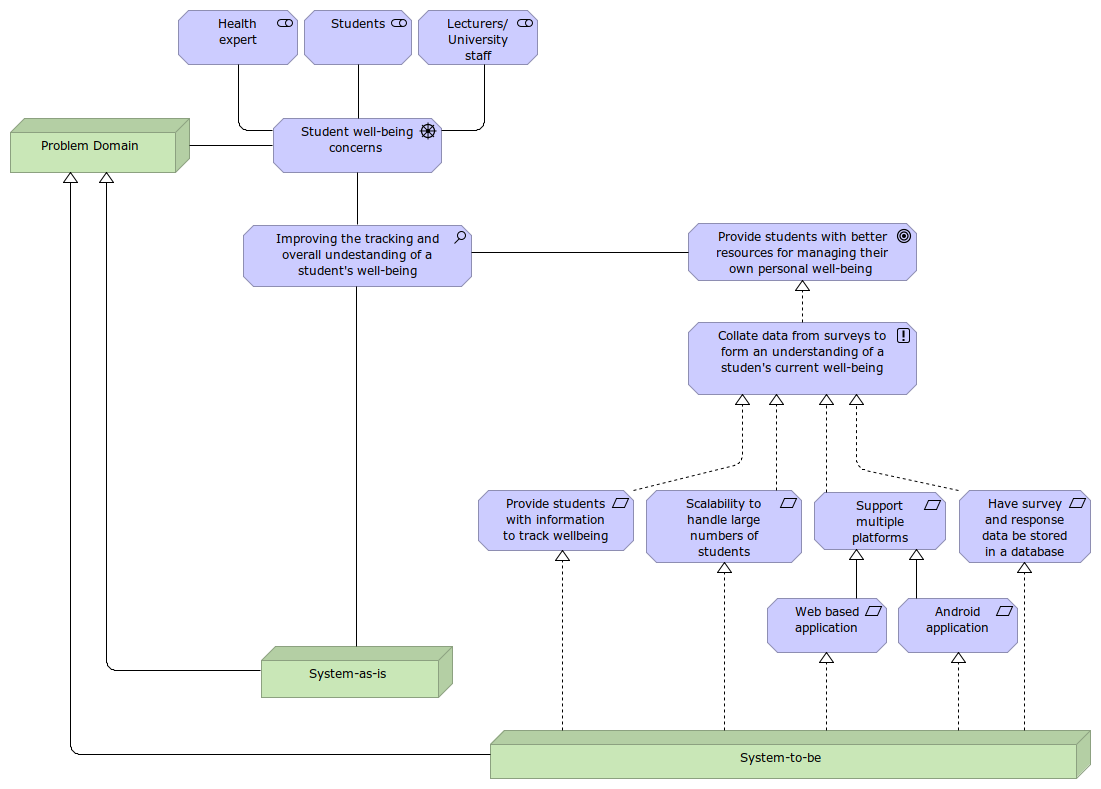
\includegraphics[width=350px]{images/motivation_model.png}
    \caption{Motivation model derived from the initial brief}
    \label{motivationmodel}
\end{figure}

\subsection{Solution-to-be}

\begin{figure}[H]
    \centering
    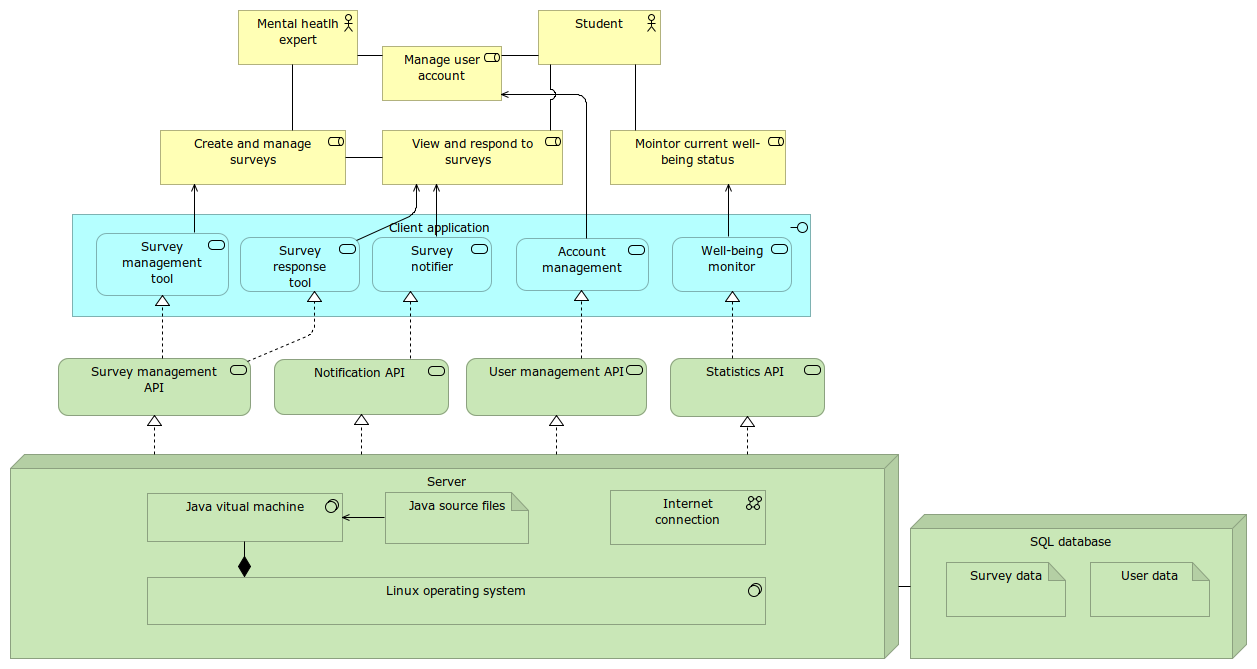
\includegraphics[width=350px]{images/solution-to-be.png}
    \caption{Proposed system solution}
    \label{solutiontobe}
\end{figure}


% Discuss the plateau-to-be/solution-to-be, specifying why it would be a good solution to the current issues with the available things already.
% The aim of this project is to provide a solution that is tailored for measuring student wellbeing. 
% In order to do this, there are some key features that need to be implemented.
For this solution to be effective, the survey creation tool needs to allow an \emph{expert} to create a survey with answers that have 
a weighted score associated with it. 
Being able to calculate an overall score allows users, both the creator and student that answered the survey, to understand the level of 
wellbeing that the student is at; identifying potential issues that may need to be addressed.
Understanding what potential issues could be present can allow a survey creator to specify resources for different scoring thresholds.
Just like other solutions, a web application would be the ideal approach as it will allow it to be used across all platforms through a web
browser.
An android application would be ideal to include, as a part of this solution, as it can allow notifications to be pushed to devices; allowing
users to know when a new survey is available to participate in.
Displaying analytic data to students, based on survey responses, can allow them to have a better way of monitoring their wellbeing.
It can also facilitate a way for people to compare their scores, and wellbeing status, with other users if they choose to as user data should be
anonymous by default.all the points covered so far, the following motivational model can be drawn out.
